\documentclass[aps, prd
, preprint
%, twocolumn
, nofootinbib 
%, notitlepage
, superscriptaddress
, longbibliography
]{revtex4-1}
\usepackage{graphicx}
\usepackage[caption=false]{subfig}
\usepackage{mathrsfs}
\usepackage{amsmath,amssymb}
\usepackage{bm}
\usepackage{braket}
\usepackage{listings}
\usepackage{cases}
\usepackage{comment}
\usepackage{soul}
\usepackage{cancel}
\usepackage{cases}
\usepackage[utf8]{inputenc}
\usepackage{url}
\usepackage{longtable}
\usepackage[normalem]{ulem}
\usepackage[colorlinks=true
,urlcolor=blue
,anchorcolor=blue
,citecolor=blue
,filecolor=blue
,linkcolor=blue
,menucolor=blue
%,pagecolor=blue
,linktocpage=true
,pdfproducer=medialab
,pdfa=true
]{hyperref}

%\usepackage{mathpazo}
%\usepackage[no-math]{fontspec}
%\setmainfont{Palatino}
%\setsansfont{Optima}

\newcommand{\dif}[2]{\frac{\mathrm{d} #1}{\mathrm{d} #2}}
\newcommand{\pdif}[2]{\frac{\partial #1}{\partial #2}}
\newcommand{\var}[2]{\frac{\delta #1}{\delta #2}}
\newcommand{\dd}{\mathrm{d}}
\newcommand{\DD}{\mathscr{D}}
\newcommand{\ee}{\mathrm{e}}
\newcommand{\diag}{\mathrm{diag}}
\newcommand{\sgn}{\mathrm{sgn}}
\newcommand{\Mpl}{M_\text{Pl}}
\newcommand{\ns}{n_{{}_\mathrm{S}}}
\newcommand{\cs}{c_{{}_\mathrm{S}}}
\newcommand{\IR}{\text{IR}}
\newcommand{\UV}{\text{UV}}
\renewcommand{\Re}{\mathrm{Re}}
\renewcommand{\Im}{\mathrm{Im}}
\newcommand{\dk}{\frac{\dd^3k}{(2\pi)^3}}
\newcommand{\bbalpha}{{\alpha\!\!\!\alpha}}
\newcommand{\dps}{\displaystyle}
\newcommand{\SIA}{S_\text{IA}}
\newcommand{\eff}{\text{eff}}
\newcommand{\kdx}{\mathbf{k}\cdot\mathbf{x}}
\newcommand{\cl}{\text{cl}}

\newcommand{\calD}{\mathcal{D}}
\newcommand{\scrD}{\mathscr{D}}
\newcommand{\uf}{\text{f}}
\newcommand{\calg}{\mathcal{g}}
\newcommand{\calH}{\mathcal{H}}
\newcommand{\scrH}{\mathscr{H}}
\newcommand{\uI}{\text{I}}
\newcommand{\calJ}{\mathcal{J}}
\newcommand{\scrJ}{\mathscr{J}}
\newcommand{\calL}{\mathcal{L}}
\newcommand{\scrL}{\mathscr{L}}
\newcommand{\calN}{\mathcal{N}}
\newcommand{\calO}{\mathcal{O}}
\newcommand{\scrO}{\mathscr{O}}
\newcommand{\calP}{\mathcal{P}}
\newcommand{\calR}{\mathcal{R}}
\newcommand{\uR}{\text{R}}
\newcommand{\uS}{\text{S}}

\newcommand{\bae}[1]{\begin{align} #1 \end{align}}
\newcommand{\bce}[1]{\begin{cases} #1 \end{cases}}
\newcommand{\bfe}[4]{
\begin{figure} 
	\centering
	\includegraphics[#1]{#2}
	\caption{#3}
	\label{#4}
\end{figure}}
\newcommand{\bpme}[1]{\begin{pmatrix} #1 \end{pmatrix}}

\newcommand{\Red}[1]{\textcolor{red}{\sffamily #1}}
\newcommand{\Mag}[1]{\textcolor{magenta}{\sffamily #1}}
\newcommand{\Blue}[1]{\textcolor{blue}{\sffamily #1}}
\newcommand{\mathblue}[1]{\textcolor{blue}{#1}}
\newcommand{\NOTE}{\textcolor{blue}{\sffamily \%\%\%\%\%\%\%\%\%\%\%\%\%\%\%\%\%\%\%\%\%\%\%\%\%\%\%\%\%\%\%\%\%\%\%\%\%\%\%\%}}



\begin{document}
\title{Noise prescription and curvature perturbations in stochastic inflation}
\date{\today}

\author{Lucas Pinol}
\email{pinol@iap.fr}
\affiliation{Institut d'Astrophysique de Paris, GReCO, UMR 7095 du CNRS et Sorbonne Universit\'e, 
98bis boulevard Arago, 75014 Paris, France}

\author{S\'ebastien Renaux-Petel}
\email{renaux@iap.fr}
\affiliation{Institut d'Astrophysique de Paris, GReCO, UMR 7095 du CNRS et Sorbonne Universit\'e, 
98bis boulevard Arago, 75014 Paris, France}

\author{Yuichiro Tada}
\email{tada.yuichiro@e.mbox.nagoya-u.ac.jp}
\affiliation{Institut d'Astrophysique de Paris, GReCO, UMR 7095 du CNRS et Sorbonne Universit\'e, 
98bis boulevard Arago, 75014 Paris, France}
\affiliation{Department of Physics, Nagoya University, Nagoya 464-8602, Japan}


\begin{abstract}
Recent works about the extension of the stochastic formalism of inflation to general multi-field models have highlighted 
the involved problem of this formalism~\cite{Pinol:2018euk,2nd}. In this formalism, the quantum diffusion of scalar fields is mimicked practically by classical white noise,
while the mathematical definition of such noise integral is arbitrary represented by the It\^o or Stratonovich integral for example.
Corresponding with this ambiguity, the equation of motion in the stochastic formalism is undetermined, strictly speaking.
In this paper, we clarify that the consequent differences in the observable curvature perturbations are fortunately negligible at least in canonical single-field cases 
with use of the analytic formulae of the stochastic-$\delta N$ formalism~\cite{Vennin:2015hra}.
Also we propose a prescription in non-canonical cases.
\end{abstract}

\maketitle
%\tableofcontents



\section{Introduction}

Inflation~\cite{Starobinsky:1980te,Sato:1980yn,Guth:1980zm,Linde:1981mu,Albrecht:1982wi,Linde:1983gd} is known as 
one of the most plausible mechanism of the early universe. It has been tested by a lot of observations and strongly supported by
e.g. the results of the Planck collaboration~\cite{Ade:2013sjv,Adam:2015rua}. Unraveling its concrete mechanism is an urgent task from the view points both of
cosmology and particle physics. On the other hand, following for example 
the possibility of primordial black holes explaining dark matters and/or gravitational wave signals announced by LIGO/Virgo
collaboration~\cite{Abbott:2016blz,Abbott:2016nmj,Abbott:2017vtc} (see e.g. Refs.~\cite{Sasaki:2018dmp}),
the quantum diffusion of scalar fields on a flat potential during inflation has recently attracted attentions (e.g. \cite{Espinosa:2017sgp,Ezquiaga:2018gbw}).
The stochastic formalism~\cite{Starobinsky:1986fx,Nambu:1987ef,Nambu:1988je,Kandrup:1988sc,Nakao:1988yi,Nambu:1989uf,Morikawa:1989xz,Mollerach:1990zf,
Linde:1993xx,Starobinsky:1994bd} is useful to investigate such a diffusion process.
In this formalism, the quantum fluctuation is mimicked by classical white noise and therefore
scalar fields' dynamics is described by the Brownian motion drifted along with their potentials
if they have. As its several aspects have been studied more and more~\cite{}, 
the stochastic formalism is of importance not only phenomenologically but also theoretically.

Even though it has been already discussed many times beyond the simplest single-field case,
recent works about the extension of the stochastic formalism to multi-field models on
general field space manifolds highlight its involved problem~\cite{Pinol:2018euk,2nd}.
Originally the definition of the integral with respect to white noise has an arbitrariness,
corresponding with the evaluation time of the noise amplitude.
In the It\^o integral, the noise amplitude is determined by the field values just before the noise kick.
As it respects the causality in this sense, this integral is adopted in several references~\cite{Salopek:1990re,Vilenkin:1999kd,Tolley:2008na,Fujita:2014tja,
Vennin:2015hra,Tokuda:2017fdh}.
However, due to the noise accumulation, the It\^o-type stochastic differential equation (SDE)
does not follow the standard chain rule, so that the equation of motion (EoM) is no longer 
covariant under the field redefinition in the It\^o's interpretation.
From the view point of the field-space covariance, the Stratonovich integral, in which 
the noise amplitude is evaluated by the middle point between before and after the noise kick,
should be adopted since its SDE follows the standard chain rule.
The authors of Ref.~\cite{Mezhlumian:1991hw} support the Stratonovich white noise as a limit of more physical
smoothed colored noise.
Unfortunately the Stratonovich integral also has a drawback that its SDE is not fixed in
the top-down approach from the quantum field theory (QFT). It depends on the choice of 
the decomposition basis of noise correlators, while QFT tells us only correlation functions.

Anyway what we observe in a current universe is not scalars' fluctuations themselves
but curvature perturbations $\zeta$ as their descendant. 
They can be calculated in the context of the
stochastic inflation with use of the so-called \emph{stochastic-$\delta N$ formalism}~\cite{Fujita:2013cna,Fujita:2014tja}.
In Ref.~\cite{Vennin:2015hra}, characteristic partial differential equations (PDE) for any moment $\braket{\zeta^n}$ are derived in this formalism
and they can be solved formally in the single-field case.
In this paper, we extend them to a general noise prescription including the It\^o and
Stratonovich integrals to investigate how the noise prescription and/or field redefinition
could affect the observable curvature perturbations indeed.

The rest of this paper is organized as follows.







\section{Drawbacks for It\^o and Stratonovich}

In the basic picture of the slow-roll inflation, the scalar inflatons $\bar{\varphi}^I$ homogeneous over the whole universe
roll down their potentials following the slow-roll equation of motion (EoM):
\bae{
	\dd \bar{\varphi}^I=-\frac{G^{IJ}V_J}{3H^2}\dd N, \qquad 3\Mpl^2H^2=V.
}
Here indices $I$ and $J$ label the inflatons, $G^{IJ}$ is the inverse of the field space metric, and $V_J$ denotes $\partial_{\varphi^J}V$.
$N$ is the e-folding number $\dd N=H\dd t$ as a time variable.
However the universe is indeed separated into each horizon patch and any superhorizon perturbation cannot be distinguished from the true homogeneous mode
by observers inside those patches. Therefore the superhorizon coarse-grained scalars should be treated as background fields instead.
Considering those coarse-grained fields, one finds that subhorizon modes join in them at every moment, exiting the horizon.
Since such modes originate from the quantum zero-point fluctuation, their effects are described well by some Gaussian noise.
Accordingly EoM for the coarse-grained fields $\varphi^I$ is modified by random kicks as
\bae{\label{eq: SR Langevin}
	\dd\varphi^I=-G^{IJ}\frac{V_J}{3H^2}\dd N + g^I_a\bullet\dd W_a,
}
where $W$'s labeled by $a$ are the independent Wiener processes representing the Brownian motion. They are as many as the inflaton fields.
The noise amplitude is given by the power spectrum of subhorizon perturbations at the horizon cross:
\bae{
	g^I_ag^J_a=\calP_\varphi^{IJ}=\frac{k^3}{2\pi^2}\int\dd^3y\Braket{\delta\varphi^I(\mathbf{x})\delta\varphi^J(\mathbf{x}+\mathbf{y})}
	\ee^{-i\mathbf{k}\cdot\mathbf{y}}.
}
These are basics of the stochastic inflation~\cite{Starobinsky:1986fx,Nambu:1987ef,Nambu:1988je,Kandrup:1988sc,Nakao:1988yi,Nambu:1989uf,
Morikawa:1989xz,Mollerach:1990zf,Linde:1993xx,Starobinsky:1994bd}.

The problem arises from the arbitrariness of the definition of noise integral $\int g^I_a\bullet\dd W_a$ when $g^I_a$ depends on the field values $\varphi^I$ themselves.
The stochastic integral for continuous time is defined by the continuous limit of the discrete sum, similarly to the standard Riemann integral, as
\bae{
	X(t)=\int^t_0A\left(X(t^\prime)\right)\bullet\dd W(t^\prime):=\lim_{\Delta t_i\to0}\sum_iA\left((1-\alpha)X_i+\alpha X_{i+1}\right)\Delta W_i.
}
Here $\alpha\in[0,1]$ parametrizes the evaluation point of the noise amplitude. Contrary to the Riemann integral, the stochastic process depends on the choice of
$\alpha$ in general. Representatively the It\^o integral indicated by the coefficient without circle $\int^t_0A\dd W$ is defined by $\alpha=0$.
This definition is preferred generally and also in the context of the stochastic inflation~\cite{Salopek:1990re,Vilenkin:1999kd,Tolley:2008na,Fujita:2014tja,
Vennin:2015hra,Tokuda:2017fdh} as the noise amplitude is determined before the noise kick itself and therefore it respects the causality.
For general $\alpha$, we use a black circle as $\int^t_0A\bullet\dd W$. Note that these integrals are convertible to each other. EoM with arbitrary 
$\alpha$~(\ref{eq: SR Langevin}) can be always rewritten with the It\^o integral as
\bae{\label{eq: Langevin in Ito}
	\dd\varphi^I=-G^{IJ}\frac{V_J}{3H^2}\dd N+g^I_a\bullet\dd W_a=\left[-G^{IJ}\frac{V_J}{3H^2}+\alpha g^J_a\partial_Jg^I_a\right]\dd N+g^I_a\dd W_a.
}

The It\^o integral, however, has an odd property, that is, it does not follow the standard chain rule.
Let us consider the field redefinition:
\bae{
	\varphi^I\to\tilde{\varphi}^A=\tilde{\varphi}^A(\varphi^I).
}
According to the It\^o's lemma~\cite{}, one must take account of the quadratic variation for its differential form as
\bae{
	\dd\tilde{\varphi}^A=\pdif{\tilde{\varphi}^A}{\varphi^I}\dd\varphi^I+\frac{1}{2}\frac{\partial^2\tilde{\varphi}^A}{\partial\varphi^I\partial\varphi^J}\dd\varphi^I\dd\varphi^J,
}
with
\bae{
	\dd W_a\dd W_b=\delta_{ab}\dd N, \qquad \dd W_a\dd N=\dd N\dd N=0.
}
Consequently one finds, after short calculations, a correction term for $\tilde{\varphi}^A$'s EoM as
\bae{\label{eq: dphiA}
	\dd\tilde{\varphi}^A=-\tilde{G}^{AB}\frac{\tilde{V}_B}{3H^2}\dd N+\tilde{g}^A_a\bullet\dd W_a
	+\left(\alpha-\frac{1}{2}\right)\tilde{\calP}_{\tilde{\varphi}}^{BC}e^A_I\partial_Be^I_C\dd N,
}
where $e^A_I=\partial\tilde{\varphi}^A/\partial\varphi^I$ and so on.\footnote{All field space indices transform tensorially like as $\tilde{O}^A=e^A_IO^I$.
		Also note the useful formula
\bae{
	e^I_B\partial_Ce^A_I=\partial_C(e^I_Be^A_I)-e^A_I\partial_Ce^I_B=\partial_C\delta^A_B-e^A_I\partial_Ce^I_B=-e^A_I\partial_Ce^I_B.
}}
It obviously means, for the It\^o's interpretation $\alpha=0$, the stochastic EoM~(\ref{eq: SR Langevin}) is no longer field-space covariant.
Since physics should not depend on the choice of the field coordinate, then the stochastic approach fails for some field definition in this case.

Eq.~(\ref{eq: dphiA}) shows that the field-space covariance remains when $\alpha=1/2$, which is called the Stratonovich integral
represented by a white circle as $\int A\circ\dd W$. 
The serious drawback of the Stratonovich integral is that, as indicated in Eq.~(\ref{eq: Langevin in Ito}), the process with $\alpha\neq0$ depends on the choice of $g^I_a$ which
is not unique in a multi-field case. Indeed the field-dependent rotation of noise basis:
\bae{
	g^I_a\to \tilde{g}^I_\alpha=R_{\alpha a}(\varphi)g^I_a, \qquad R^T_{a\alpha}R_{\alpha b}=\delta_{ab},
}
changes EoM~(\ref{eq: Langevin in Ito}) even though it does not affect the power spectrum itself, 
$\tilde{g}^I_\alpha\tilde{g}^J_\alpha=g^I_ag^J_a=\calP_\varphi^{IJ}$.\footnote{Strictly speaking, one must show that the It\^o integral $\int g^I_a\dd W_a$ itself is not affected 
by the noise rotation to prove the basis dependence of the whole equation. However to see the Fokker-Planck equation corresponding with 
Eq.~(\ref{eq: Langevin in Ito}) would be the fastest way:
\bae{
	\partial_NP=-\partial_I\left[\left(-G^{IJ}\frac{V_J}{3H^2}+\alpha g^J_a\partial_Jg^I_a\right)P\right]+\frac{1}{2}\partial_I\partial_J\left(\calP_\varphi^{IJ}P\right).
}
It shows that only EoM in the It\^o's interpretation is independent of the choice of noise basis.}
Any physical valid theory does not tell the decomposition choice since physics should depend only on the correlators,
and therefore this noise basis is not determined in a top-down approach.
Note that it matters only in multi-field cases since there is no degree of freedom (d.o.f.) of basis rotations, while
the It\^o's problem remains also for a single-field model because one can always redefine even the single field.

Even though we pointed out drawbacks both for the It\^o and Stratonovich integrals, it would be a naturally arising question whether
these indeed alter the observable signals. The typical observables of inflation is not the fluctuation of the inflaton fields themselves but the conserved curvature perturbations.
The so-called stochastic-$\delta N$ formalism has been proposed as a prescription to calculate curvature perturbations in the stochastic approach~\cite{Fujita:2013cna,
Fujita:2014tja,Vennin:2015hra}. In the next section, we investigate the impact on the curvature perturbations of the choice of noise integral and the field redefinition
with use of this method.








\section{Analytic formulae for curvature perturbations}

The stochastic formalism is a powerful tool to investigate the fluctuations of scalar fields. However the observables which we can detect now are not themselves 
but the curvature perturbations. In Refs.~\cite{Fujita:2013cna,Fujita:2014tja}, the algorithm to calculate the power spectrum of the curvature perturbations has been proposed
by combining the stochastic formalism and the $\delta N$ formalism, and then it is dubbed the stochastic-$\delta N$ approach.
The authors of Ref.~\cite{Vennin:2015hra} formulate it in terms of partial differential equations and show the formal solution in a single-field case.
This work adopts the It\^o's interpretation. Then, in this section, we first extend this formulation to a general noise integral in Sec.~\ref{sec: stochastic-delta N}
to see the effect of the choice of noise interpretation on the curvature perturbation. We also see the impact of field redefinition in Sec.~\ref{sec: field redefinition}.





\subsection{Stochastic-$\delta N$ formalism}\label{sec: stochastic-delta N}

To calculate the curvature perturbations on superhorizon scales, the $\delta N$ formalism~\cite{Starobinsky:1986fxa,Salopek:1990jq,Sasaki:1995aw,Sasaki:1998ug,
Lyth:2004gb}. According to this formalism, the curvature perturbations are equivalent to the spatial variation of the e-folding numbers from some initial flat slice
to the final uniform-density slice. This fluctuation of e-foldings is denoted by $\delta N$, originating the formalism's name.
Interestingly, the stochastic formalism automatically makes the e-folding numbers probabilistic. It is encoded as a first passage time to the final slice
and its stochastic distribution has all information of curvature perturbations.

If the inflaton fields follow the stochastic EoM~(\ref{eq: Langevin in Ito}),
some calculations in stochastic calculus reveal that the $n$th moment $f_n(\varphi)=\braket{\calN^n}(\varphi)$ of the first passage time $\calN$ from
an initial field value $\varphi$ to some boundary 
(which should correspond with the final uniform-density slice) satisfies the following recursive partial differential equation (PDE):
\bae{\label{eq: fn PDE}
	\left[\left(-G^{IJ}\frac{V_J}{3H^2}+\alpha g^J_a\partial_Jg^I_a\right)\partial_I+\frac{1}{2}\calP_\varphi^{IJ}\partial_I\partial_J\right]f_n=-nf_{n-1},
}
with $f_0=1$ and the absorbing boundary condition (b.c.) $f_n|_\text{boundary}=0$, $(n\ge1)$.\footnote{See Ref.~\cite{Vennin:2015hra} and appendices of 
Ref.~\cite{Assadullahi:2016gkk} for a detailed derivation.} Directly PDE for the variance $g_2=\braket{\delta\calN^2}=\braket{\calN^2}-\braket{\calN}^2=f_2-f_1^2$
follows as
\bae{\label{eq: g2 PDE}
	\left[\left(-G^{IJ}\frac{V_J}{3H^2}+\alpha g^J_a\partial_Jg^I_a\right)\partial_I+\frac{1}{2}\calP_\varphi^{IJ}\partial_I\partial_J\right]g_2
	=-\calP_\varphi^{IJ}(\partial_If_1)(\partial_Jf_1),
}
with the same b.c. $g_2|_\text{boundary}=0$.

Even though they are merely one point functions, one can extract the two point function, i.e., the power spectrum of the curvature perturbations.
Assuming that all perturbations exit the horizon between the initial and final time, the variance of $\delta\calN$ (or curvature perturbation $\zeta$) can be related with
its power spectrum as
\bae{
	\braket{\delta\calN^2}=\int_{k_\uf\ee^{-\braket{\calN}}<k<k_\uf}\dk P_\zeta(k)\ee^{i\mathbf{k}\cdot\mathbf{0}}
	=\int_{\log k_\uf-\braket{\calN}}^{\log k_\uf}\calP_\zeta(k)\dd\log k,
}
where $\calP_\zeta(k)=\frac{k^3}{2\pi^2}P_\zeta(k)$ is the dimensionless power spectrum and $k_\uf$ is a horizon scale on the final slice.
Inversely the power spectrum is derived as
\bae{
	\calP_\zeta(k)=\left.\dif{\braket{\delta\calN^2}}{\braket{\calN}}\right|_{k=k_\uf\ee^{-\braket{\calN}}}.
}
Obviously $\calP_\zeta=g_2^\prime/f_1^\prime$ in single-field cases.

The strong point of this method is that it automatically includes all resummation effects on superhorizon scales. At the price of this merit,
the recursive PDE is generally difficult to solve analytically, and even numerically.
However, in single-field cases, it reduces to ordinary differential equations which can be solved at least formally.
For a canonical single field and in the slow-roll approximation as $3\Mpl^2H^2=V$ and $\calP_\varphi=\left(\frac{H}{2\pi}\right)^2$, Eq.~(\ref{eq: fn PDE}) reads
\bae{
	\left(-\frac{v^\prime}{v}+\alpha v^\prime\right)f_n^\prime+vf_n^{\prime\prime}=-n\frac{f_{n-1}}{\Mpl^2}, \qquad v=\frac{V}{24\pi^2\Mpl^4},
}
which can be solved as
\bae{\label{eq: fn}
	f_n(\varphi)=n\int^\varphi_{\varphi_\uf}\frac{\dd x}{\Mpl}\int^{\bar{\varphi}_n}_x\frac{\dd y}{\Mpl}\frac{f_{n-1}(y)}{v^\alpha(x)v^{1-\alpha}(y)}
	\exp\left[\frac{1}{v(y)}-\frac{1}{v(x)}\right],
}
where $\bar{\varphi}_n$ is a constant of integration so that $v(y)>v(x)$.\footnote{It corresponds with the reflecting b.c. $f^\prime_n(\bar{\varphi}_n)=0$ at some high potential point 
$\bar{\varphi}_n$. Practically it should not affect the resultant moment $\braket{\calN^n}$ so much for a realistic initial field value $\varphi$.}
PDE for $g_2$ also reduces to
\bae{
	\left(-\frac{v^\prime}{v}+\alpha v^\prime\right)g_2^\prime+vg_2^{\prime\prime}=-2v{f_1^\prime}^2,
}
and it is solved as
\bae{\label{eq: g2}
	g_2(\varphi)=2\int^\varphi_{\varphi_\uf}\dd x\int^{\tilde{\varphi}_2}_x\dd y\left(\frac{v(y)}{v(x)}\right)^\alpha{f_1^\prime}^2(y)\exp\left[\frac{1}{v(y)}-\frac{1}{v(x)}\right].
}
Again $\tilde{\varphi}_2$ is a constant of integration.

They are still far from easy-understanding.
Here note that the energy scale of realistic inflationary models should be sufficiently lower than the Planck scale as $v(x)<v(y)\ll1$ and therefore the integrands have main contributions only around $y\sim x$ due to the exponential suppression $\exp\left[\frac{1}{v(y)}-\frac{1}{v(x)}\right]$.
Then, taking the Taylor expansion of the exponent around $x$ as
\bae{
	\frac{1}{v(y)}-\frac{1}{v(x)}\simeq-z+\left.\left(v-\frac{v^2v^{\prime\prime}}{2{v^\prime}^2}\right)\right|_xz^2+\cdots, \qquad z=\left.\frac{v^\prime}{v^2}\right|_x(y-z),
}
we will consider linear corrections in $v$ and $\eta_\cl=v^2v^{\prime\prime}/{v^\prime}^2$.
Similarly,
\bae{
	\frac{1}{v^\alpha(x)v^{1-\alpha}(y)}\simeq\frac{1}{v}\left(1-(1-\alpha)vz+\cdots\right),
}
and then one obtains, up to $\calO(v,\eta_\cl)$,
\bae{\label{eq: f1 saddle}
	f_1(\varphi)\simeq\int^\varphi_{\varphi_\uf}\frac{\dd x}{\Mpl^2}\frac{v}{v^\prime}\left(1+(1+\alpha)v-\eta_\cl\right).
}
One should here note that the slow-roll EoM for a homogeneous background gives the well-known formula of e-foldings as $N_\cl(\varphi)=\int^\varphi_{\varphi_\uf}\frac{\dd x}{\Mpl^2}\frac{v}{v^\prime}$.
Therefore the second and third terms in the parenthesis of Eq.~(\ref{eq: f1 saddle}) represents the stochastic resummation effect which makes the mean e-folds $\braket{\calN}$ deviate from the homogeneous value.
While $v=V/24\pi^2\Mpl^4$ should be always small, $\eta_\cl=v^2v^{\prime\prime}/{v^\prime}^2$ can be large for a sufficiently flat potential and it would be an index parameter of stochasticity~\cite{Vennin:2015hra}.\footnote{This parameter is written as $\eta_\cl=\frac{1}{2}\eta_V\calP_{\zeta,\cl}$ with use of the second slow-roll parameter $\eta_V=\Mpl^2\frac{v^{\prime\prime}}{v}$ and the slow-roll formula $\calP_{\zeta,\cl}=\frac{2}{\Mpl^2}\frac{v^3}{{v^\prime}^2}$ for the power spectrum of curvature perturbations. Both of them are basically small but $\eta_V$ can be larger than unity in a limited region like as an inflection point model for example~[\Blue{Garcia-Belido}]}

Similarly one obtains
\bae{\label{eq: g2 saddle}
	g_2(\varphi)\simeq2\int^\varphi_{\varphi_\uf}\frac{\dd x}{\Mpl^4}\frac{v^4}{{v^\prime}^3}\left(1+(6+3\alpha)v-5\eta_\cl\right),
}
and then the power spectrum of curvature perturbations reads
\bae{\label{eq: calP saddle}
	\calP_\zeta\simeq\calP_{\zeta,\cl}\left(1+(5+2\alpha)v-4\eta_\cl\right),
}
with the standard slow-roll formula $\calP_{\zeta,\cl}=\frac{2}{\Mpl^2}\frac{v^3}{{v^\prime}^2}$.
Also, with use of $\partial/\partial\log k\simeq=-\partial\varphi/\partial\braket{\calN}\times\partial/\partial\varphi$ at leading order in slow-roll, the spectral index is given by
\bae{\label{eq: ns saddle}
	\ns-1=\pdif{\log\calP_\zeta}{\log k}=-\frac{g_2^{\prime\prime}}{f_1^\prime g_2^\prime}+\frac{f_1^{\prime\prime}}{{f_1^\prime}^2}\simeq n_{{}_\text{S},\cl}-1+\left(-2(2+\alpha)\epsilon_V+3\eta_V\right)v-6\eta_V\eta_\cl+8\epsilon_V\xi_\cl.
}
Here $n_{{}_\uS,\cl}=1-6\epsilon_V+2\eta_V$ is a standard one and $\epsilon_V$ and $\eta_V$ are the slow-roll parameters as
\bae{
	\epsilon_V=\frac{\Mpl^2}{2}\frac{{v^\prime}^2}{v^2}, \qquad \eta_V=\Mpl^2\frac{v^{\prime\prime}}{v}.
}
We also introduced another stochasticity parameter $\xi_\cl=v^3v^{\prime\prime\prime}/{v^\prime}^3$ assumed as small as $\eta_\cl$.

Interestingly all $\alpha$-dependences (that is, the noise integral dependences) are suppressed by $v\ll1$ irrespectively of the stochasticity parameters $\eta_\cl$ and $\xi_\cl$.
It suggests that the choice of noise integral hardly affect the curvature perturbations even where the stochastic resummation effect is large. 
In the rest of this subsection, we resort to the numerical approach to check it, directly calculating the formal solutions~(\ref{eq: fn}) and (\ref{eq: g2}).

%%%%%%%%%%%%%%%%%%%%
\begin{figure}
	\centering
	\begin{tabular}{cc}
		\begin{minipage}{0.5\hsize}
			\centering
			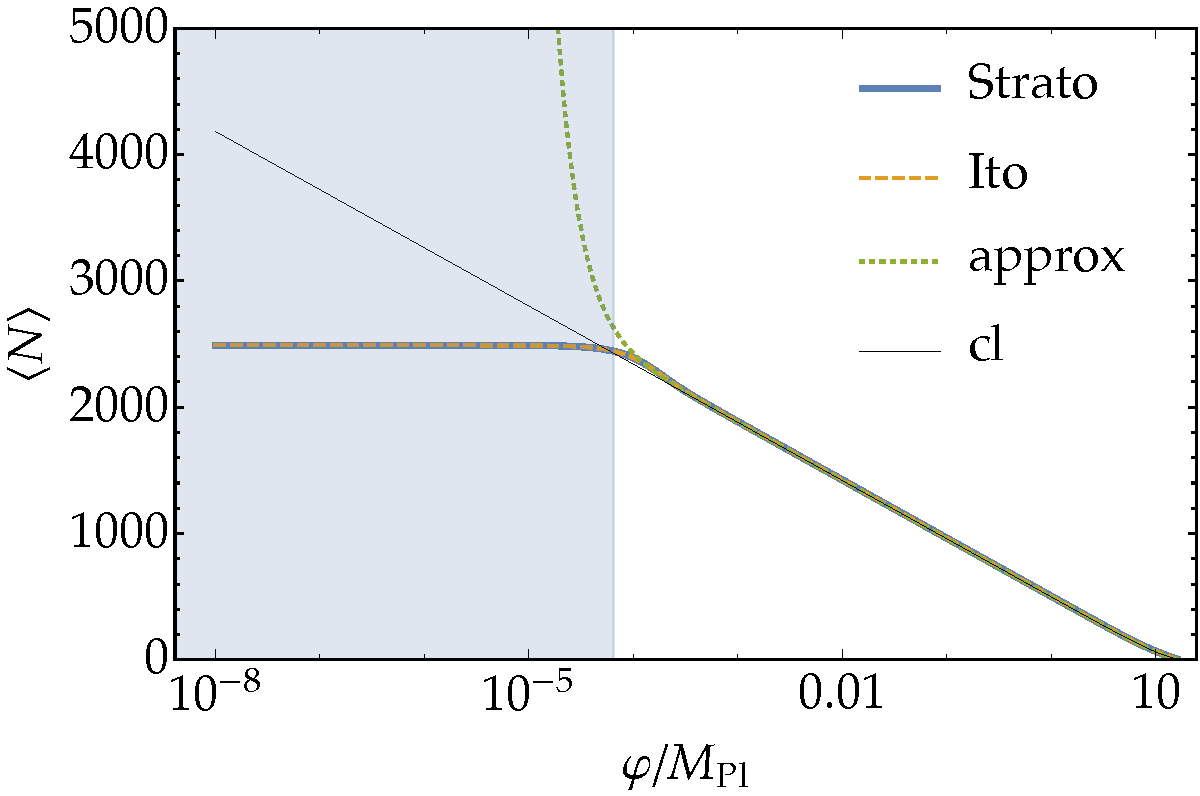
\includegraphics[width=\hsize]{figs/N.pdf}
		\end{minipage}
		\begin{minipage}{0.5\hsize}
			\centering
			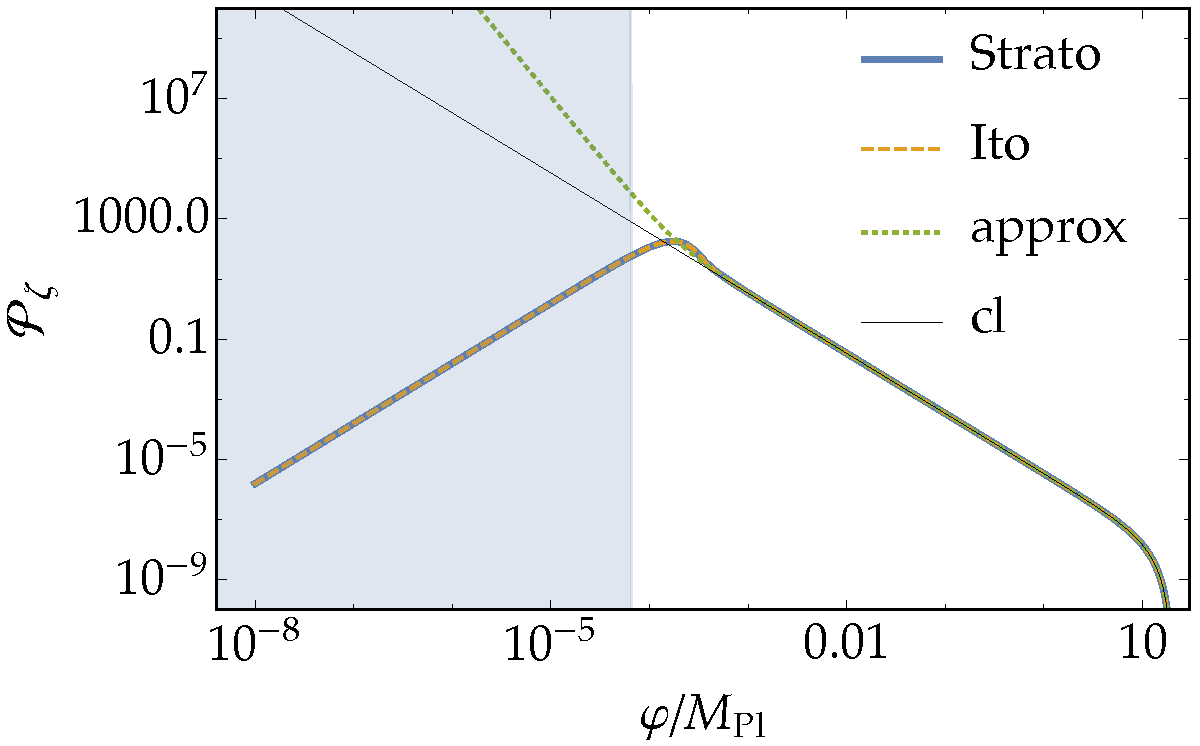
\includegraphics[width=\hsize]{figs/calP.pdf}
		\end{minipage} \\[100pt]
		\begin{minipage}{0.5\hsize}
			\centering
			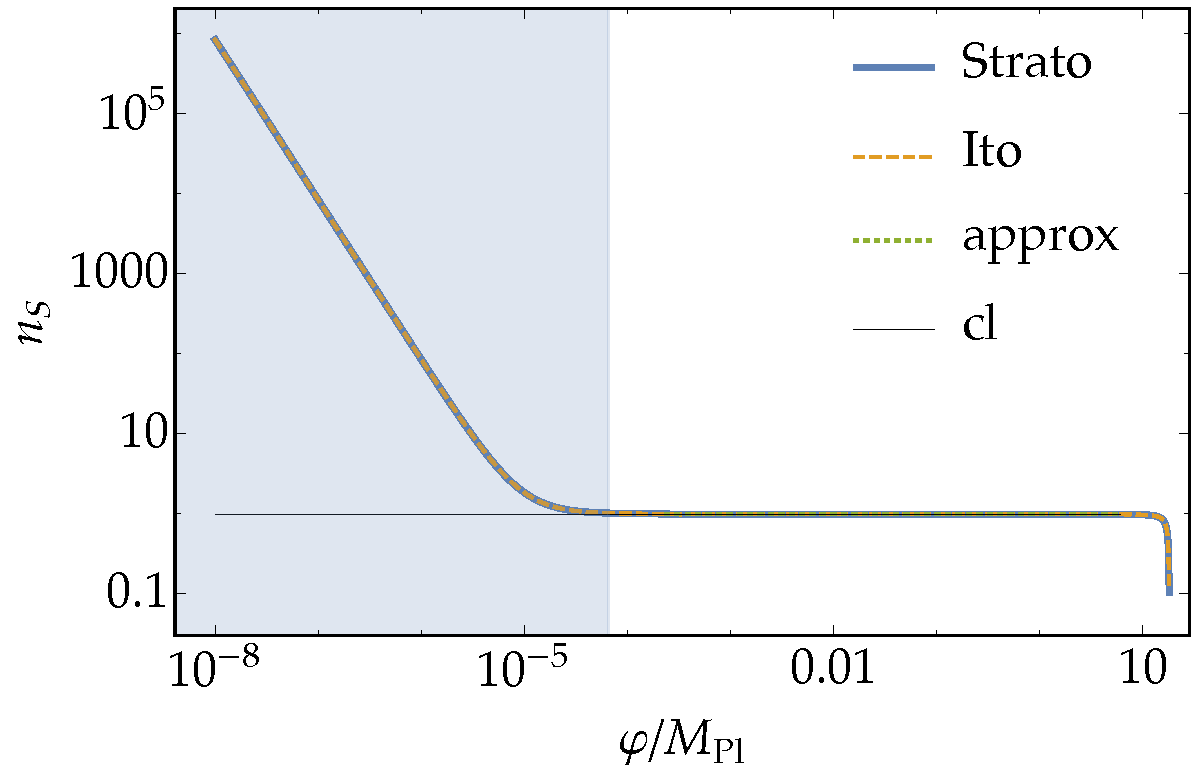
\includegraphics[width=\hsize]{figs/ns.pdf}
		\end{minipage}
		\begin{minipage}{0.5\hsize}
			\centering
			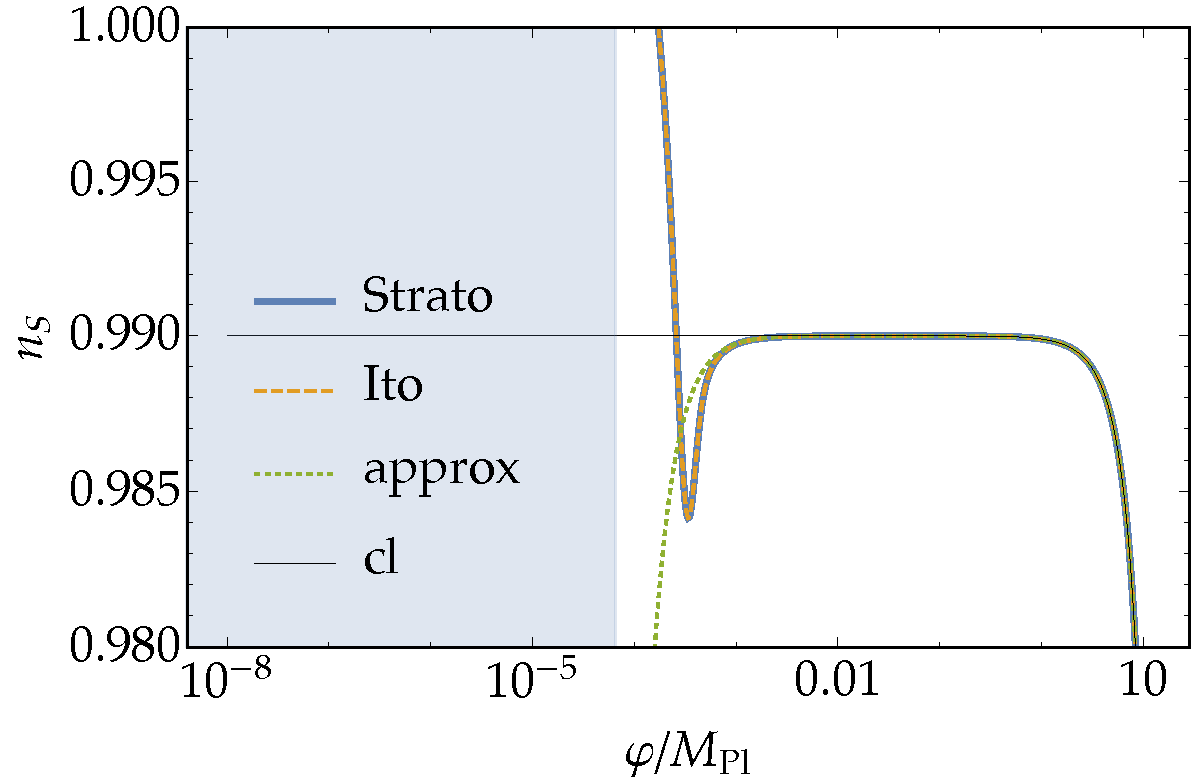
\includegraphics[width=\hsize]{figs/ns_mag.pdf}
		\end{minipage}
	\end{tabular}
	\caption{Numerical results by full expressions (\ref{eq: fn}) and (\ref{eq: g2}) in Stratonovich $\alpha=1/2$ (“Strato”) and It\^o $\alpha=0$ (“Ito”), 
	approximated expansions (\ref{eq: f1 saddle}), (\ref{eq: calP saddle}), and (\ref{eq: ns saddle}) in Stratonovich $\alpha=1/2$ (“approx”), 
	and the standard formulae (“cl”). The classicality condition $|\eta_\cl|\ll1$ is violated in shaded regions. We choose the constants of integration as 
	$\bar{\varphi}_1=\tilde{\varphi}_2=0$.}
	\label{fig: hilltop}
\end{figure}
%%%%%%%%%%%%%%%%%%%%

Fig.~\ref{fig: hilltop} shows the mean e-folds, the power spectrum of curvature perturbations, and its spectral index for hilltop inflation with the following potential.
\bae{
	V(\varphi)=\Lambda^4\left(1-\frac{\varphi^2}{\mu^2}\right), \qquad \Lambda=10^{-2}\Mpl, \qquad \mu=20\Mpl.
}
The full results in the stochastic-$\delta N$ formalism by the formal solutions~(\ref{eq: fn}) and (\ref{eq: g2}) are exhibited with the approximated expansions~(\ref{eq: f1 saddle}), (\ref{eq: calP saddle}), and (\ref{eq: ns saddle}), and the standard slow-roll formulae.
In shaded regions, the classicality condition $|\eta_\cl|\ll1$ is violated and therefore the stochastic effect cannot be neglected.
First one can check that both the full solutions and approximated expansions in the stochastic-$\delta N$ are well consistent with the standard formulae, validating the parameter $\eta_\cl$ as the criterion of the stochasticity.
Also it should be noted that, though the stochastic results start to deviate from the standard ones when $|\eta_\cl|>1$ showing large stochastic resummation effects, the difference between the It\^o and Stratonovich integrals is still negligible as suggested.
Accordingly, at least in canonical single-field cases,
it is indicated that the effect of the choice of noise integral on the observable curvature perturbations can be neglected.




\subsection{Field redefinition}\label{sec: field redefinition}

While there is no d.o.f. of vielbein rotations in single-field cases and the Stratonovich's difficulty resolves, 
one still has the d.o.f. of the field redefinition causing the It\^o's problem. Then let us investigate the effect of field redefinitions on curvature perturbations in this subsection.

Considering the field redefinition from the canonical scalar $\varphi$ to the non-canonical one $\psi$, the field-space metric for $\psi$ 
is given by $G_{\psi\psi}=e^{-2}$ where $e=\partial\psi/\partial\varphi$.
Before solving the momenta $\braket{\calN^n}$, let us first consider the slow-roll condition for the new field $\psi$.
In the curved field space, it is given by
\bae{
	|D_t\dot{\psi}|=|\ddot{\psi}+\Gamma^\psi_{\psi\psi}\dot{\psi}^2|\ll|H\dot{\psi}|,
}
where $D_t$ represents the covariant time derivative $D_t\calO^I=\partial_t\calO^I+\Gamma^I_{JK}\dot{\varphi}^J\calO^K$.
Then both $|\ddot{\psi}|$ and $|\Gamma^\psi_{\psi\psi}\dot{\psi}^2|$ are assumed to be much smaller than $|H\dot{\psi}|$ unless an accidental cancelation.
With use of $\Gamma^\psi_{\psi\psi}=-e_\psi/e$ and the slow-roll background EoM $3H\dot{\psi}\simeq-e^2V_\psi$,
one obtains
\bae{
	\left|\frac{\Gamma^\psi_{\psi\psi}\dot{\psi}^2}{H\dot{\psi}}\right|=\left|\Mpl^2\frac{ee_\psi v_\psi}{v}\right|\ll1.
}
Accordingly we refer to this as a new slow-roll parameter $\tilde{\eta}_\psi=\Mpl^2\frac{ee_\psi v_\psi}{v}$ for $\psi$.
One can also obtain another slow-roll parameter by decomposing the original one as
\bae{
	\eta_{\varphi}=\Mpl^2\frac{v_{\varphi\varphi}}{v}=\Mpl^2\frac{e\partial_\psi(ev_\psi)}{v}=\eta_\psi+\tilde{\eta}_\psi,
}
where we defined $\eta_\psi=\Mpl^2\frac{e^2v_{\psi\psi}}{v}$. 
Both $\eta_\psi$ and $\tilde{\eta}_\psi$ can be naturally assumed to be small.

Let us also estimate the form of the classicality conditions for $\psi$. Similarly to the original classicality parameter 
$\eta_{\phi,\cl}=v^2v_{\varphi\varphi}/v_\varphi^2=\frac{1}{2}\calP_{\zeta,\cl}\eta_\varphi$, 
we consider the product of the classical power spectrum
and the slow-roll parameter as
\bae{
	\tilde{\eta}_{\psi,\cl}:=\frac{1}{2}\calP_{\zeta,\cl}\eta_\psi=\frac{1}{\Mpl^2}\frac{v^3}{e^2v_\psi^2}\times\Mpl^2\frac{ee_\psi v_\psi}{v}
	=\frac{e_\psi v^2}{ev_\psi}.
}
It should be small enough in a realistic case as $\calP_{\zeta,\cl}$, $\eta_\psi\ll1$. Again decomposing the original classicality parameter, one obtains another one:
\bae{\label{eq: decomposition of eta_phicl}
	\tilde{\eta}_{\varphi,\cl}=\frac{v^2v_{\varphi\varphi}}{v_\varphi^2}
	=\frac{v^2e\partial_\psi(ev_\psi)}{e^2v_\psi^2}=\eta_{\psi,\cl}+\tilde{\eta}_{\psi,\cl},
}
where $\tilde{\eta}_{\psi,\cl}=v^2v_{\psi\psi}/v_\psi^2$.
Finally the other classicality parameter $\xi_{\varphi,\cl}$ is rewritten by $\psi$ as
\bae{
	\xi_{\varphi,\cl}=\frac{v^3v_{\varphi\varphi\varphi}}{v_\varphi^3}=\xi_{\psi,\cl}+\tilde{\xi}_{\psi,\cl}
	+\frac{1}{v}\tilde{\eta}_{\psi,\cl}^2+\frac{3}{v}\eta_{\psi,\cl}\tilde{\eta}_{\psi,\cl},
}
where $\xi_{\psi,\cl}=\frac{v^3v_{\psi\psi\psi}}{v_\psi^3}$ and
$\tilde{\xi}_{\psi,\cl}=\frac{e_{\psi\psi}v^3}{ev_\psi^2}$.
The last two terms are $\calO(\eta_{\varphi,\cl})$ and therefore the first two terms $\xi_{\psi,\cl}$ and
$\tilde{\xi}_{\psi,\cl}$ should be also as small as $\calO(\eta_{\varphi,\cl})$ if one assumes 
$\xi_{\varphi,\cl}\sim\calO(\eta_{\varphi,\cl})$. 

For a non-canonical field $\psi$, the general formulae~(\ref{eq: fn PDE}) and (\ref{eq: g2 PDE}) reduce to
\bae{
	\bce{
		\dps
		\left[\left(-e^2\frac{v_\psi}{v}+\alpha(e^2v)_\psi\right)\partial_\psi+e^2v\partial_\psi^2\right]f_n=-n\frac{f_{n-1}}{\Mpl^2}, \\[10pt]
		\dps
		\left[\left(-e^2\frac{v_\psi}{v}+\alpha(e^2v)_\psi\right)\partial_\psi+e^2v\partial_\psi^2\right]g_2=-2e^2v{f_{1,\psi}^2},
	}
}
which can be solved as
\bae{\label{eq: general fn and g2}
	\bce{
		\dps
		f_n(\psi)=n\int^\psi_{\psi_\uf}\frac{\dd x}{\Mpl}\int^{\bar{\psi}_n}_x\frac{\dd y}{\Mpl}\frac{f_{n-1}(y)}{(e^2(x)v(x))^\alpha(e^2(y)v(y))^{1-\alpha}}
		\exp\left[\frac{1}{v(y)}-\frac{1}{v(x)}\right], \\[10pt]
		\dps
		g_2(\psi)=2\int^\psi_{\psi_\uf}\dd x\int^{\tilde{\psi}_2}_x\dd y\left(\frac{e^2(y)v(y)}{e^2(x)v(x)}\right)^\alpha{f_{1,\psi}^2}(y)
		\exp\left[\frac{1}{v(y)}-\frac{1}{v(x)}\right].
	}
}
$f_1$ and $g_2$, as intended, can be expanded with use of the derived classicality parameters as
\bae{
	\bce{
		\dps
		f_1(\psi)\simeq\int^\psi_{\psi_\uf}\frac{\dd x}{\Mpl^2}\frac{v}{e^2v_\psi}\left(1+(1+\alpha)v-2(1-\alpha)\tilde{\eta}_{\psi,\cl}-\eta_{\psi,\cl}\right), \\[10pt]
		\dps
		g_2(\psi)\simeq2\int^\psi_{\psi_\uf}\frac{\dd x}{\Mpl^4}\frac{v^4}{e^4{v_\psi}^3}\left[1+(6+3\alpha)v-5\eta_{\psi,\cl}-2(3-\alpha)\tilde{\eta}_{\psi,\cl}\right].
	}
}
They can be rewritten in terms of $\varphi$ by the change of the integration variable $x\to\tilde{x}$ so that $\partial x/\partial\tilde{x}=e$, 
and keeping the relation~(\ref{eq: decomposition of eta_phicl}) in mind, one obtains
\bae{
	\bce{
		\dps
		f_1(\psi)\simeq\int^{\varphi(\psi)}_{\varphi(\psi_\uf)}\frac{\dd\tilde{x}}{\Mpl^2}\frac{v}{v_\varphi}
		\left(1+(1+\alpha)v-\eta_{\varphi,\cl}-(1-2\alpha)\tilde{\eta}_{\psi,\cl}\right), \\[10pt]
		\dps
		g_2(\psi)\simeq\int^{\varphi(\psi)}_{\varphi(\psi_\uf)}\frac{\dd\tilde{x}}{\Mpl^4}\frac{v^4}{{v_\varphi}^3}\left[1+(6+3\alpha)v-5\eta_{\varphi,\cl}
		-(1-2\alpha)\tilde{\eta}_{\psi,\cl}\right],
	}
}
They obviously reproduce the canonical results~(\ref{eq: f1 saddle}) and (\ref{eq: g2 saddle}) if and only if $\alpha=1/2$.
That is, except in the Stratonovich interpretation, the stochastic EoM~(\ref{eq: SR Langevin}) and then the corresponding PDE~(\ref{eq: fn PDE}) and (\ref{eq: g2 PDE})
are not invariant under the field redefinition, and therefore the non-canonical definition of field leads to different results from those for the canonical field.

The correction terms for $f_1$ and $g_2$ are canceled by each other in the expression of the power spectrum and therefore it remains unchanged 
from Eq.~(\ref{eq: calP saddle}) as
\bae{
	\calP_\zeta=\frac{g_{2,\psi}}{f_{1,\psi}}=\frac{g_{2,\varphi}}{f_{1,\varphi}}\simeq\calP_{\zeta,\cl}\left(1+(5+2\alpha)v-4\eta_{\varphi,\cl}\right),
}
while the spectral index is varied since the e-folds correspondence $f_1$ is shifted:
\bae{
	\ns=&\,1-\frac{g_{2,\psi\psi}}{f_{1,\psi}g_{2,\psi}}+\frac{f_{1,\psi\psi}}{f_{1,\psi}^2} \nonumber \\
	=&\,n_{{}_\text{S},\cl}+\left(-2(2-\alpha)\epsilon_V+(3-2\alpha)\eta_V\right)v-6\eta_V\eta_{\varphi,\cl}+8\epsilon_V\xi_{\varphi,\cl} \nonumber \\
	&-3(1-2\alpha)\tilde{\eta}_{\psi}v+2(1-2\alpha)\eta_V\tilde{\eta}_{\psi,\cl}.
}
It again reduces to the canonical result~(\ref{eq: ns saddle}) only if $\alpha=1/2$.

These corrections are not suppressed by $v$, so the results can significantly depend on the field definition in highly stochastic cases 
except in the Stratonovich approach, contrarily to
the physical intuition. Even though the calculation in the canonical definition seems to be natural, one cannot conclude which definition gives correct results, 
speaking strictly, because the top-down approach from the first principle is also broken down and cannot be used for comparison in stochastic regions.
Then let us here reconsider the meaning of the difference between the It\^o and Stratonovich integrals.
The difference is expressed by $g^J_a\partial_Jg^I_a$ as can be seen in Eq.~(\ref{eq: Langevin in Ito}) or (\ref{eq: fn PDE}).
It can be naively interpreted as the variation of $I$-noise due to the noise kick itself. Therefore it indicates the self-interaction of noise.
On the other hand, since we assumed that the noise can be approximated to be Gaussian, this variation term should be smaller than the $I$-noise itself for the validity of that anzats.
That is, the following condition can be used for a check of the proper choice of the field definition and vielbein, and the smallness of the intrinsic non-Gaussianity:
\bae{
	\frac{g^J_a\partial_Jg^I_a}{\sqrt{g^I_bg^I_b}}\ll1,
}
where the $I$'s summation is not taken. In the single test field case, it reduces to
\bae{
	\left|\frac{g\partial_\psi g}{g}\right|=\left|\partial_\psi\left(e\frac{H}{2\pi}\right)\right|=\left|\frac{H}{2\pi}e_\psi\right|=\left|\sqrt{2\tilde{\eta}_\psi\tilde{\eta}_{\psi,\cl}+\epsilon_Vv}\right|\ll1.
}
As $v$ is always small, this condition constrains $\tilde{\eta}_{\psi,\cl}$ not to be large.
Therefore, with this condition, the difference between canonical and non-canonical results will be neglected and then the It\^o-Stratonovich problem does not matter, too.
According to this logic, the canonical ($e=1$) results which always satisfy this condition become reliable, and also one can always use, if he/she wants, 
the Stratonovich integral which does not depend on the field definition.

Also note that this condition does not necessarily mean the low stochasticity. Even if some stochasticity parameter like $\eta_{\psi,\cl}=v^2v_{\psi\psi}/{v_\psi^2}$
is large, $\tilde{\eta}_{\psi,\cl}=e_\psi v^2/(ev_\psi)$ can be small with the canonical field being a good example.
Therefore the stochastic calculation in the large stochasticity region can be valid as long as the field is chosen so that $|\partial_\psi g|\ll1$,
and it is rather a necessary method in such a case. 








\section{Conclusions}




%\acknowledgments





%\appendix







\bibliography{main}
\end{document}



